\documentclass[fr]{../../../eplsummary}

\renewcommand{\labelitemi}{$\bullet$}
\renewcommand{\labelitemii}{$\cdot$}
\renewcommand{\labelitemiii}{$\diamond$}
\renewcommand{\labelitemiv}{$\ast$}

\usepackage[french]{varioref} % \vref and \vpageref
\usepackage{graphicx} % images
\usepackage{float} % images
\usepackage{url}
	\urlstyle{sf}
\usepackage[backgroundcolor=yellow]{todonotes} %% todonotes: \listoftodos & \todo{Some note or other.} & \missingfigure{}

% draw
\usepackage{tikz}
\usetikzlibrary{arrows}
% \usepackage{qtree}    % dessiner des arbres %% => texlive-humanities

\definecolor{codeBlue}{rgb}{0,0,1}
\definecolor{webred}{rgb}{0.5,0,0}
\definecolor{codeGreen}{rgb}{0,0.5,0}
\definecolor{codeGrey}{rgb}{0.6,0.6,0.6}
\definecolor{webdarkblue}{rgb}{0,0,0.4}
\definecolor{webgreen}{rgb}{0,0.3,0}
\definecolor{webblue}{rgb}{0,0,0.8}
\definecolor{orange}{rgb}{0.7,0.1,0.1}

\usepackage{caption}
\renewcommand{\familydefault}{\sfdefault}

\usepackage{listings}		% Pour l'insersion de fichiers de codes sources.
\lstset{
	  language=Java,
	  frame=single,
	  flexiblecolumns=true,
	  numbers=none, % left
	  stepnumber=1,
	  numberstyle=\ttfamily\tiny,
	  keywordstyle=\ttfamily\textcolor{blue},
	  stringstyle=\ttfamily\textcolor{red},
	  commentstyle=\ttfamily\textcolor{green},
	  breaklines=true,
	  extendedchars=true,
	  basicstyle=\ttfamily\scriptsize,
	  showstringspaces=false
	}

\lstdefinelanguage{diff}{
  morecomment=[f][\color{blue}]{@@},     % group identifier
  morecomment=[f][\color{red}]-,         % deleted lines
  morecomment=[f][\color{green}]+,       % added lines
  morecomment=[f][\color{magenta}]{---}, % Diff header lines (must appear after +,-)
  morecomment=[f][\color{magenta}]{+++},
}

\IfFileExists{fourier.sty}{\usepackage{fourier}}{\typeout{! WARNING: Fourier package not included: skip it}}

%%%%%%%%%%%%%%%%%%%%


\title{LINGI2172 - Exams}
\author{Matth, LN, Alex, Ben, Leader, Houtain Nicolas}
\hypertitle{Databases}{8}{INGI}{2172}
{Houtain Nicolas \and Matthieu Baerts\and Benoît Baufays\and Julien Colmonts\and Alex Vermeylen\and Hélène Verhaeghe}
{Bernard Lambeau}
\section{Intro}
A database is a collection og related data, where data means fact that
can be stored and have an implicit meaning. Key point are:
\begin{itemize}
	\item Focus on information, not only storage.
	\item Independence (weak coupling for easier maintenance)
	\item High-level Specification, there is a guarentee on the behavior
	(because of the ACID property).
	\item Information aims at being queried.
\end{itemize}
According to the book:
\begin{description}
	\item[A database] is an organized machine readable collection of symbols
	 (we can see the value of the database) and machine-updatable.
\end{description}
\section{Lexique}
\begin{itemize}
	\item Variable : C'est une représentation à un temps t de la fonction. La ``table''
	    représente plutôt la valeur de variable.

	    Represent a predicate.
	\item[Notes:] Une table $\neq$ relation puisque la relation est indépendante
	    de l'ordre des rows/columns.

    \item Relation : Fonction qui lie les attributs entre eux. 
    C'est elle qui leurs donne un sens.
    \item Attribut : Un champ de la variable
    \item Cardinalité :  Nombre de n-tuple
    \item N-Tuple : une ligne, un ensemble d'attribute value
    \item Tuple : ensemble des lignes
    \item Orthogonalité : %TODO
\end{itemize}


\section{DBMS}
The DBMS is a piece of software for managing databases and providing
access to them. It has several function such as:
\begin{itemize}
	\item Create and destroy variable
	\item Assuring data integrity rules (constraint)
	\item Update variable
	\item ...
\end{itemize}
\begin{figure}[H] 
    \centering
    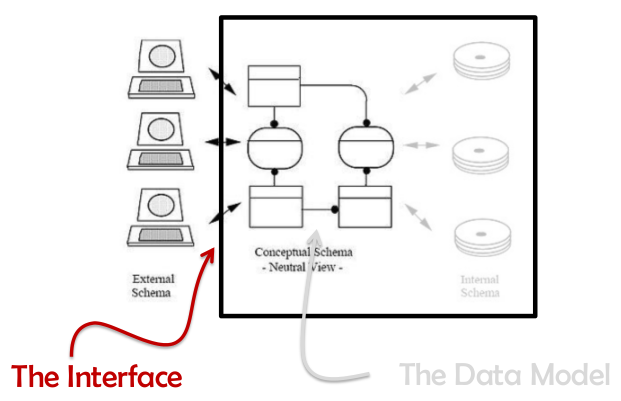
\includegraphics[width=10cm]{img/dbms.png}
    \caption{Database design}
\end{figure}
Everything is kept hidden, only information is exposed to the software layer.
\begin{description}
    \item[DML] : Data Manipulation Language (manipulate data)
    \item[DDL] : Data Definition Language (manipulate schema, metadata)
\end{description}

\section{Predicate logique}
A predicat is the meaningor a certain kind of sentence, but often used
to refer to the sentece itself.
\paragraph{Note :} By sentence, we means sentences with the form of
a statement (can be true of false). Notice that the meaning is 
language-independant while the sentence is not.
\\
Une proposition est composé de différent paramètre (ex: $x \leq y$).
P(x), a predicate, is called a membership
predicate for the set consisting of all such objects a.

\begin{itemize}
    \item[Definition]
    \item Intension : its meaning
    \item Extension : all the instantiations that are ''true''
    \item Substitution : replace a paramerter by a \textit{designator}
    \item Instantiation : substitution of all the parameter
    \item N-adic predicate : A predicate with n parameters.
    \item[Operator]
    \item Conjunction, disjunction , negation, implication, only if, equivalence

    \item[Quatifiers]
    \item Existential, universal

    \item[Sets]
    \item $\in$, $\subseteq$, $\supseteq$, $\subset$, $\supset$, equality
    \item Join, disjointness, union, intersection, complement, difference
\end{itemize}


A \textbf{relation} represents the extension of some n-adic predicate P,
by having a body consisting of every n-tuple that satisfies P.
\subsection{Tutorial D}
\subsubsection{Foundation}
There are important distinctions in Tutorial D that must be explained
given the example \texttt{Y : = X + 1} :
\begin{description}
	\item[Value vs variable: ] Y denotes a variable, X denotes the value 
	currently assigned to the variable X. 1 denotes a value. Variables
	are subject to change while value exists independently of time.
	\item[Variable vs variable reference: ] X and Y are both referencing 
	variable, but the context makes them denote different thing. 
	\item[Update operator versus read-only operator: ] ''\texttt{:=}'' is 
	an update operator (UO) and ''\texttt{+}'' is a read-only operator
	(ROO). An UO has at least on parameter that is subject to update
	which is not the case for a ROO. But a ROO yields a value.
	\item[Operator vs invocation: ] ''\texttt{+}'' is an operator and
	\texttt{X + 1} is an invocation of this operator.
	\item[Parameter vs argument: ] An argument refers to the substitution
	of the defined parameter of the operator by values. (\texttt{X and 1}
	are arguments of the operator \texttt{+} which is defined to have 2 
	parameters.
	\item[Parameter subject to update vs parameter not subject to update: ]
	Update operator \texttt{:=} take two parameters. The first one
	is subject to update so it must be substitute by a variable. The second
	one is no subject to update so it must be substitute by a value.
\end{description}
\subsubsection{Relation Type}
A type (= domain) is a named set of values. The value in the sets are
called litteral. The type of a relation is defined by its heading.\\
It's possible in Tutorial D to define user-type that are a subtype
system existing type. 
\begin{lstlisting}
TYPE SID POSSREP SID { C CHAR
			CONSTRAINT LENGTH(C) <= 5
				AND
			  	STARTS_WITH(C,'S')
				AND
				IS_DIGIT(SUBSTRING(C,1)))
			 }
	INIT SID(`S1');
\end{lstlisting}
\begin{table}
    \centering
    \begin{tabular}{|l|l|}
        \hline
        \textbf{Logic} & \textbf{Tutorial D} \\
        \hline
        AND & JOIN \\
        & WHERE (restriction) \\
        & EXTEND (extension) \\
        & SUMMARIZE \\
        \hline
        EXISTS & EXISTS (projection) \\
        \hline
        OR & UNION \\
        \hline
        (AND) NOT & MINUS (difference) \\
        & NOT MATCHING (semi-difference) \\
        \hline
        & RENAME \\
        \hline
    \end{tabular}
    \caption{Link Logic operate and Tutorial D}
\end{table}

\subsubsection{JOIN}

Let $s = r_1 JOIN r_2$.
$\to$ Commutative and associative.


\paragraph{Special case :}
\begin{itemize}
    \item R JOIN R = \textbf{R}
    \item If all attributes are common to both operand = \textbf{Intersection}
    \item If no attribute are common to both operand = \textbf{Cartesian product}
\end{itemize}

\subsubsection{EXISTS}
Let $s = r \{A_1, \cdots, A_n\} = r\{ ALL BUT \quad B_1, \cdots, B_m\}$.

\paragraph{The heading of s} = the subset of the heading of r given by $\{A_1, \cdots, A_n\}$.

\paragraph{The body of s} = each tuple that can be formed
from a tuple of r by removing from it the attributes named $\{B_1, \cdots, B_m\}$.

\paragraph{Special case :}
\begin{itemize}
    \item $R \{ ALL BUT \}$ = \textbf{R}
    \item $R \{ \}$ = \textbf{A relation with no attributes at all}
\end{itemize}


\subsubsection{WHERE}
Let $s = R WHERE C$

\paragraph{Special case :}
\begin{itemize}
    \item $R WHERE TRUE$ = \textbf{R}
    \item $R WHERE FALSE$ = \textbf{A empty relation with heading of R}
\end{itemize}

\subsubsection{ TODO }

TODO slide 4b

\subsection{PostgreSQL}

\subsubsection{Tuple Calculus and Relational Algebra }
A tuple relational calculus have the form:
$${t_1.A_j,t_2.A_k,...,t_n.A_m|COND(t_1...t_n)}$$ 
\paragraph{Example:} \{t.Fname,t.Lname,t.Address | EMPLOYEE(t) AND ($\exists d$)(DEPARTMENT(d)
AND d.Dname = 'Research' AND d.Dnumber = t.Dno\} which corresponds to a query listing the name and 
address of all employees who work fot the 'Research' department.\\
While in relational algebra you build the solution (X = 98+2) , in Tuple
calculus you describe it (find x s.t X-2=98).

\subsubsection{SQL relationnal operator}

\begin{table}
    \centering
    \begin{tabular}{|l|l|}
        \hline
        \textbf{Logic} & \textbf{SQL} \\
        \hline
        AND & JOIN \\
        & WHERE (restriction) \\
        & GROUP BY  (HAVING)\\
        \hline
        EXISTS & EXISTS (projection) \\
        & DISTINCT\\
        & IN\\
        \hline
        OR & UNION \\
        \hline
        (AND) NOT & EXCEPT (difference) \\
        &NOT EXISTS\\
        & NOT IN (semi-difference) \\
        \hline
        & AS \\
        \hline
    \end{tabular}
    \caption{Link Logic operate and SQL}
\end{table}

%TODO EXAMPLE WITH 5b slide 30 WHERE FAILS

\section{Constraint}

Constraints express the integrity rules for a database.
They enforcement of constraints by the DBMS ensures that the
database is at all times in a consistent state.

\subsection{KEY constraints}%\label{key}
A key for a relvar r is a set of attributes of r (i.e, a subset of 
r's heading) such that at no time does r contain more than one tuple
having any given collection of valuers for those attributes.\\
A key must have the property of irreducibility meaning that we cannot 
take any attribute away from a key and still have a key.\\
A relvar can have several keys : the nominated one is called 
''primary key'' and the others ''alternate keys''.

\paragraph{Definition from the book}
\begin{description}
	\item[SuperKey :] Let K be a subset of a ther heading of the relvar $r$. Then K is a 
	\textbf{superkey} for $r$ iff , at all times , t1 and t2 both appear
	in the body of $r$ and the projection t1\{K\} is equal to the
	projection t2\{K\},then t1 = t2(i.en they are the same tuple)
	\item[Key :] K is \textbf{key} for $r$ iff:
	 \begin{itemize}
	 	\item K is a superkey for $r$
	 	\item No proper subset of K is a superkey for $r$.
	 \end{itemize}
\end{description}

In others word, a superkey is a set of attributes that uniquely identifies
any tuples within the body of the relvar. A superkey become a key 
when it is reduced to the minimum number of attributes.

\subsection{Foreign key}

There is a \textbf{inclusion dependency} because the relation which
contains a foreign key (SECOND) must be included into the relation which
contains the key (FIRST) : $$ FIRST\ { StudentId } \supseteq SECOND \ {
StudentId}$$



\paragraph{Generalisation of inclusion dependency}
$$ IS\_EMPTY( SECOND\ NOT\ MATCHING\ FIRST )$$

\paragraph{Multiple assignement} is used when we need to update several
variable on the same time to respect some constraint.

\subsection{Implicit constraint}

A single relvars (which describe ``A'' like : ID\#, Name, Field1,
Field2) have an implicit constraint to the effect that every ``A'' has a
ID, a Name, a Field1 and a Field2\ldots

To avoid this implicit constaint, we need to decomposed the design in
different table link by the a foreign key (ID\#).

\paragraph{ }
The single relvar design is preferred so long as the constraint implied
by it truly reflects the real world!

\section{Normal Form}
In database design, there are some requirement that can be used to check 
the quality of database:
\begin{itemize}
	\item Orthogonality
	\item Redundancy
	\item Simplicity
\end{itemize}

\subsection{Fonctional dependency (FD)}\label{fd}

Soit une relation $R$, un set d'attributs (\textbf{determinant}) et
détermine un set (\textbf{dependant set}) $\forall (x \rightarrow y)$
si et seulement si chaque valeur de $x$ est associée à un élément de
$y$. Note that a FD denotes a function.

For example, in the relation $a+b=c$ we have $\{a,b\} \rightarrow \{c\}$.

\paragraph{Theorem about FD: }
\begin{itemize}
    \item Left augmentation : if A' is a superset of A, then A' $\to$ B 
    \item Right reduction : if B' is a subset of B, then A $\to$ B' 
    \item Transivity : if A $\to$ B and B $\to$ C, then A $\to$ C 
    \item General : if A $\to$ B and C $\to$ D, then A $\cup ( C - B) \to B \cup D$
    \item[]
    \item Left-irreducibility : if A $\to$ B and there is no proper subset A' such
        that A' $\to$ B, then A $\to$ B is \textbf{left-irreducible} and B is said
        \textit{fully dependent} on A.
    \item[]
    \item A is a superkey of r if A $\to$ B and A $\cup$ B constitutes the entire
        heading of r
    \item A is a key of r if A $\to$ B is left-irreducible and A $\cup$ B constitutes the entire
        heading of r
\end{itemize}

\subsection{Join dependency}\label{jd}

Une relation est sujette à une join dependency si elle peut être
recréée en joignant plusieurs tables ayant chacune un sous ensemble
des attributs de la relation.

On parle de \textit{join dependency triviale} si une des tables du join
à tous les attributs de la relation initiale: bref que l'on ne peut
plus faire de join dependency (voir exemple en section \vref{6NF}).
\paragraph{Notation:}
Si on a la relvar \texttt{WIFE\_OF\_HENRY\_VIII}  = \{Wife\#,FName,LName,Fate\}
, une JD se note : * \{ \{ Wife\#,FName \}, \{Wife\#, LName , Fate \}\}


\subsection{Normalisation}
Normalisation is the act of decomposing a relvar that fails
to satisfy a given normal form scuh that the result is an
equivalent set of two or more ''smaller'' relvars that do satisfy
that normal form. The goal of the normalisation are:
\begin{itemize}
	\item Remove redundancy
	\item No update anomalies
	\item Full orthogonality
\end{itemize}

\subsection{1 NF}
\paragraph{Normalisation}

A relation is in 1NF if attribute domains include only
atomic (simple, indivisible) values and each tuple
attribute value is a single value from the domain.

% http://www.tablesgenerator.com/#
% http://truben.no/latex/table/
\begin{table}[H]
\begin{tabular}{|c|c|c|}
\hline
A$_1$ & A$_2$ & A$_3$ \\ \hline
      &       &       \\ \hline
      &       &       \\ \hline
\end{tabular}
\hfill
\begin{tabular}{|c|c|c|}
\hline
A$_1$ & A$_2$ & A$_3$ \\ \hline
      &   \rule{0pt}{3ex} \begin{tabular}{|c|c|}\hline & \\ \hline \end{tabular}    &       \\ \hline
      &   \rule{0pt}{3ex} \begin{tabular}{|c|c|}\hline & \\ \hline \end{tabular}    &       \\ \hline
\end{tabular}
\hfill
\begin{tabular}{|c|c|c|}
\hline
A$_1$ & A$_2$ & A$_3$ \\ \hline
      &   \rule{0pt}{5ex} \begin{tabular}{|c|}\hline \\\hline \\ \hline \end{tabular}    &       \\ \hline
      &   \rule{0pt}{5ex} \begin{tabular}{|c|}\hline \\\hline \\ \hline \end{tabular}    &       \\ \hline
\end{tabular}
\end{table}

The first is good, but in the second there is no atomic value (there is a tuple)
and in the third we have no simple value.

\subsection{3 NF}
Source: Wikipédia.\\
Doit premièrement être 2 NF: tout attribut \textit{non-prime} (donc pas dans une clé) doit dépendre d'une clé entière (pas juste certains attributs).

Ensuite, tout \textit{non-prime} ne peut être transitivement dépendant ($A \rightarrow B, B \rightarrow C$: $C$ est transitivement dépendant de $A$) de toutes super keys de R.\\

On peut également définir par cette définition : Pour toute dépendance fonctionnelle ($X \rightarrow A$), il doit y avoir au moins une de ces 3 conditions qui soit correcte:
\begin{itemize}
	\item $X$ contient $A$ ($A\subseteq X$)  (FD triviale, voir section \vref{fd})
    \item $X$ est une superkey (voir section \vref{key})
    \item chaque élément de $A \backslash \{X\}$ est \textit{prime} (est contenu dans une clé)
\end{itemize}

For example go check \url{http://www.studytonight.com/dbms/database-normalization.php}

\subsection{BCNF}
Pour toutes dépendances fonctionnelles (voir section \vref{fd}) $X \rightarrow A$, il doit y avoir au-moins une de ces 2 conditions respectées:
\begin{itemize}
	\item $X$ contient $A$ ($A\subseteq X$)  (FD triviale, voir section \vref{fd})
    \item $X$ est une superkey (voir section \vref{key})
\end{itemize}

BCNF allows to deal with the redundancy and the lack of orthogonality 
through splitting.

\subsection{5 NF}
Une relation est 5NF si toutes \textit{join dependencies} (voir section \vref{jd}) non-triviales est implicite par les candidate keys (= super key quand il n'y a pas encore de clé primaire): \textit{join dependencies} à $\{A, B, ..., Z\}$ est implicite par les candidates keys si et seulement si chaque $A, B, ..., Z$ est superkey.

\subsection{6 NF}\label{6NF}
Une relation est 6NF si elle ne satisfait aucune \textit{join dependency} (autre que les triviales donc).\\

\begin{table}[H]
\begin{center}
\begin{tabular}{|l|l|l|l|l|l|l|l|}
\cline{1-2} \cline{4-5} \cline{7-8}
\textbf{ID} & \textbf{FName} & \textbf{} & \textbf{ID} & \textbf{LName} & \textbf{} & \textbf{ID} & \textbf{Status} \\ \cline{1-2} \cline{4-5} \cline{7-8}
1           & Alex           &           & 1           & Vermeylen      &           & 1           & Sleeping        \\ \cline{1-2} \cline{4-5} \cline{7-8}
2           & LN             &           & 2           & Verhaeghe      &           & 2           & Watching TV     \\ \cline{1-2} \cline{4-5} \cline{7-8}
\end{tabular}
\caption{Exemple de 6NF}
\end{center}
\end{table}
On ne peut plus faire de join dependency mais du coup, c'est dangereux: si on ajoute une nouvelle entrée dans la première table, il faut ajouter des contraintes pour être sûr d'ajouter aussi dans les autres tables si c'est nécessaire.

\subsection{FD-driven Logical Design}
A general method for logical design is
given a relvar R with heading H and some FDs, decompose R into
relvars $R_1\  ...\  R_n$ s.t
\begin{itemize}
	\item $H\ =\ H_1\cup\ ...\ \cup\ H_n$
	\item $R_i$ is in a particular NF, $\forall i$
	\item Every FD appears in a $R_i$
	\item R = JOIN\{$R_1,\ ...\ ,R_n$\}
\end{itemize}

\subsection{Heath's theorem}
\begin{itemize}
	\item Let A,B and C be subsets of the heading of a relvar R s.t every 
	attribute appears in at least one subset and suppose FD $A\to B$ 
	holds.
	\item Then , the JD*$\{A\cup B,A\cup C\} $holds in R
\end{itemize}

%%TODO Algorithms

\section{View, Rules \& Triggers}

\subsection{View}

View are computed relation variables (capture predicate extension, 
should be updatable, have constraints and have keys). 

But, unlike ''BASE'', they should be kept hidden to end-users.
Views allows the independence of the logical schema. If the schema
evolves (i.e for a better design), views will shield users from
breaking changes.

%TODO

\subsubsection{View updating}
\begin{description}
	\item[Golden rule :] No database is ever allowed to violate its 
	own databas constraint.
	\item[Assigment principle :]After assignment og value v to 
	variable V then v = V must evaluate to true.
\end{description}
Depending on how the view is defined, updating a view can be a problem.
For example:
\begin{lstlisting}
V := SUPPLIERS{CITY} UNION PARTS {CITY}
\end{lstlisting}
If we want to insert something, do we have to do it in the both?

\subsection{Rules \& Triggers}

Both of them are object in database but trigger be attached to a 
relvar.

%TODO :
Ce sont tous les deux des objets de base de données mais les
triggers sont attachés à une table et uniquement déclanché après
qu'un \texttt{INSERT}, un \texttt{UPDATE} ou un \texttt{DELETE} ait
été utilisé. Donc en gros, c'est pour exécuter une requête
automatiquement lorsqu'un tel événement a lieu. Attention, ceci peut
être fait avant ou après (à spécifier à la création du trigger),
donc pas forcément à postériori mais en tous cas, le trigger ne
modifie pas l'AST! (et il ne peut donc pas annuler des opérations, etc.
alors qu'avec un \textit{rule}, on peut avec \texttt{INSTEAD NOTHING})\\

Alex (en parlant de Triggers vs. \textbf{Rules}): Je dirais plus que la
différence principale c'est que le trigger ne se déclenche réellement
qu'après que l'insert (ou autre opération) ait été achevé ; alors
que la rule elle, modifie l'AST (arbre représentant l'execution plan
pour une query) et donc, le code produit pour faire la query est
différent et tient compte de cette rule.

De ce fait, la rule est plus efficace que le trigger. Si on fait 100
insert, on exécute 100 fois le trigger ; alors que si on modifie
l'arbre, on ne doit construire qu'une seule fois cet arbre. Le travail
est donc le même pour une ou 100 query(ies).

En outre, la rule peut être utilisé avec une view, alors que le
trigger, ne peut pas.

\section{Database programming}
\begin{table}[H]
\centering
\begin{tabular}{|c|c|c|c|}
\hline
\textbf{Techinique} & \textbf{Examples} & \textbf{What is exposed} & \textbf{Data transfer}\\
\hline
Active Database & PSM,PL/SQL& SQL code& Shared variables and cursors\\
\hline
Embedded SQL &&SQL code & Shared variables and cursors\\
\hline
Call-level APIs&JDBC,ODBC&SQL as string repr.&Cursor-like ResultSet\\
\hline
Query builders& Sequel,JOOQ& SQL ASTs&Cursor-like ResultSet\\
\hline
ORMS&Hibernate & Object model & Class instances(one at a time)\\
\hline
First-class Relation &Alf & Relations and Relvars& Relation instances (set at a time)\\
\hline
\end{tabular}
\caption{Various approaches to Database Programming}
\end{table}
An host language is a language in which SQL calls are embedded.
%TODO table slide 9c (64)
\subsection{Active database} 
SQL with statement, trigger and stored procedures

\begin{itemize}
    \item Branching/loops : IF .. THEN .. ELSE, WHILE .. DO .., REPEAT.. UNTIL ..
    \item Interaction :SELECT .. INTO .., Cursors
\end{itemize}
A cursors is a tuple-variable that ranges over all tuples in the result 
of some query. We can get the result from the cursor through the 
\texttt{FETCH} command.
\begin{itemize}
    \item[Pros]
    \begin{itemize}
		\item Easy to use \& deploy.
		\item Efficiency (treaments close to data)
		\item Transactions made easy
     \end{itemize}
     \item[Cons]
    \begin{itemize}
		\item Difficult to test \& deploy (incompatibility)
		\item Hard to scale/distribute processing
		\item Bad programming language design
	\end{itemize}
\end{itemize}

\subsection{Embedded SQL}
In Embedded SQL a preprocessor is used. SQL statements are turned into
procedure calls that fit with the host-language code surronding. (Key word
EXEC is used to easiliy recognize SQL calls\\
To interact with each other,  SQL and the host-language share variable. 
Embedded SQL is no longer used because it is hard to maintain programs with 
mixed styles and there is a need for higher-level construts.

\subsection{Call-level interface} 
Use a external library to connect and execute some statement on
the database. It's a low level because the query is write into
a String and pass as argument to a function which return a result set.

\begin{itemize}
    \item[Pros]
    \item Standardize at the API level, keep the control (because low-level)
    \item[Cons]
    \item SQL injection risks, difficult to maintain
\end{itemize}

\subsection{Query builder} 
Query is like a object and we can execute some function (where(), join(), select(),...)
on the table to have some result.

This idea raise the level of abstraction (no visible string concatenation, 
handles SQL escaping automatically)

\begin{itemize}
    \item[Pros]
    \item Cleaner that previous solution, easier for dynamically created queries,
        less prone to SQL injection
    \item[Cons]
    \item Complex queries tend to be a mess to build
\end{itemize}

\subsection{ORM} 
Expose a Class diagram(Object model) instead of a relational schema to 
the application layer. Then map that diagram to the relational schema. 
\begin{itemize}
    \item[Pros]
    \begin{itemize}
		\item Simple and less prone to SQL injections
		\item Natural data layer for object-minded people
	\end{itemize}
    \item[Cons]
    \begin{itemize}
		\item OO/ Relation Mismatch (one-at-a-time vs set-at-at-a-time ways of thinking)
		\item Software coupling (Huge OO model where all is already implemented
		\item Require control of the SQL schema
		\item Hide database connections and transaction
	\end{itemize}
        %TODO
\end{itemize}

\subsection{Relation as first-class citizen}
Expose relation concepts at application layer (relational algebra)
\begin{itemize}
	\item[Pros]
	\begin{itemize}
		\item Algebra cleaner than SQL query builders
		\item Simpler and sounder %%SOunder?
	\end{itemize}
	\item[Cons]
	\begin{itemize}
		\item Risk of loosing control of generated SQL.
		\item Not widely available.
	\end{itemize}
\end{itemize}

\subsection{The NOSQL Cases}
Data models is not the same: Key-value stores or document database. With one
of these approach, it is easier to do a mapping with a programming languages.

\section{Transactions}
\subsection{Purposes}
DBMS manages database variables, the variable are:
\begin{itemize}
	\item Mutable : different values at different times.
	\item Shared : read \& updated by many users or processes
	at the same time.
	\item Complex: consistency constraints to be preserved whatever
	happens.
\end{itemize}
Mutable shared state is one of the biggest source of complexity in
software engineering. Transaction deals with this problem.
\subsection{Properties}
Toutes les transactions doivent être ACID pour être relationnelles. ACID:
\begin{itemize}
    \item \textbf{Atomic}: The whole process is done or none is.
    \item \textbf{Concistant}: Database constraints are preserved.
    \item \textbf{Isolated}: Appear to the user as if only one process executes at a time.
        (Need to manage with concurrence)
    \item \textbf{Durability}: Effect of a process do not get lost\ldots 
        Modifications are permanent.

\end{itemize}

There is Read-only and Read-write access for a transaction\ldots Indeed, using 
this may improve performance in practice.

\paragraph{ } Use COMMIT to complete the transaction or ROLLBACK to abort
the transaction.


\subsection{Isolation levels}

\begin{tabular}{|l|c|c|c|}
    Level & Dirty read & Nonrep. read & Phantom read \\
    \hline
    Serializable (safest) & x & x & x \\
    Repeatable read & x & x & v \\
    Read committed & x & v & v \\
    Read uncommitted (unsafest) & v & v & v \\
    \hline
\end{tabular}

Serializable is the most safe solution because the observable 
result is the same as if T1 and T2 were serial\ldots but it's not 
the most efficient solution.

\begin{itemize}
    \item Dirty read : Read of data written by a concurren uncommited transaction.
    \item Nonrepeatable read : re-read data and find it has been updated by
        another transaction that committed since the initial read.
    \item Phtantom read : re-read and sees new inserted/deleted record by
        another transaction that commited since the initial read.
\end{itemize}

\section{Recovery}
\subsection{Aim of Recovery}

There are different type of failure such as system failures,  
transaction failures and media
failures. The aim of recovery is to ensure \textbf{atomicity} 
(revert all transaction updates),\textbf{consistency} (roolback from a 
inconsistent state) and \textbf{durability}.


\subsection{Transaction log}

The key problem is the unfinished transaction ! The solution
is to use a transaction log and on failure recovery, unfinished transaction
have start but no commit nor abort record.

Three solution to make the transaction log :
\begin{itemize}
    \item Undo logging (immediate changes) :
    \item[Drawback] : Cannot commit transaction without lots of I/O and
        cannot use the log to bring backup database copies up to date.
    \item[]
    \item Redo logging (deferred changes) :
    \item[Drawback] : Need to keep all modified block in memory until commit.
    \item[]
    \item Both of them
\end{itemize}
\subsubsection{Undo logging}
The idea is to keep old value in the log records and do the real update 
job on disk. Operation can be undo on failure recovery thanks to the log.
(see example slide 16 in 10c)
\subsubsection{Redo logging}
The idea is to keep new values in log recodes and do the real update on
in memory (not the disk!). Because update are not done on the disk,
opetation can be redo on failure recovery thanks to the log.
%TODO explain undo and redo and undo/redo

\paragraph{Checkpointing the log} to avoid very long transaction logs.
So periodically :
\begin{enumerate}
    \item Do not accept new transactions
    \item Wait until all transaction finish
    \item Flush all log record to disk
    \item Flush all buffers to disk
    \item Write ``checkpoint'' record on disk
    \item Resume transaction processing
\end{enumerate}
When a recovery must be done, it starts at the last checkpoint.
\subsection{Media failures}
%TODO
To cope with with Media Failure, there is no choice but making copies.
There are different techniques:
\begin{itemize}
	\item Triple redundancy (keep 3 copies on separate disks)
	\item Redundant writes/single reads
	\item Backup database + log
\end{itemize}


\section{Concurrency control}

A process can \textbf{read(X)} and \textbf{write(X)} without any assumption
on the sceduler.

\subsection{Transaction Schedule}
Two differents transactions are in conflict if they want to do an
operation on the same data item and one of the operation is a write.\\
Transation execute concurrently in an interleaved fashion, the order 
of execution in which they operates is known as the transaction
scedule. 
\subsection{Serializability}
\paragraph{Serial schedule}
For every transaction T participating in the schedule, all the
operations of T are executed consecutively in the schedule.
\paragraph{Serializable schedule}
A schedule S is serializable :
\begin{itemize}
	\item if it is equivalent to some serial 
	schedule of the same n transactions
	\item Allow interleaving of transcation operations
\end{itemize}
Serial and serializable schedule are correct (consistency of database).
\subsection{Equivalences} %TODO ameliorer explication
\begin{description}
	\item[Result equivalent ] They produce the same final state of the
	database
	\item[Conflict equivalent] The order of any two conflicting operations
	 is the same in both schedules
	\item[Conflict serializable] Conflict equivalent to some serial schedule.
	(It can be tested throug a directed graph (slide 15 in 11a))
\end{description}
\subsubsection{Lock}
Lock and unlock need to be atomic operation.

\begin{itemize}
    \item[MODES]
    \item Read lock (X) : More than one transaction can share read lock on X but
        no write lock on X by other transaction
    \item Write lock (x) : only one write lock on X
    \item[CONVERSION]
    \item Lock upgrade : read lock on X to write lock on X (Need to have only
        one read lock on X)
    \item Lock downgrade : from write lock on X to read lock on X
\end{itemize}

\paragraph{Transactions requirement}
A transaction should be well-formed : lock data before access them, does not lock 
an already locked data item and not try to unlock an unlocked data item.

\subsubsection{Two-phase locking}
\begin{enumerate}
    \item Growing phase : Transaction applies locks on desired data item
        \begin{itemize}
            \item lock data one at a time
            \item incrementally lock during execution (but may cause deadlock)
            \item All-or-nothing locks before transactions begins execution
        \end{itemize}
    \item Shrinkin phase : Transaction unlock ressource
\end{enumerate}

\subsubsection{Deadlock}
The scheduler maintains a \textbf{wait-for-graph} and if he detect a cycle
then a deadlock exist. In this case, one transaction involved in the cycle
is selected and rolled-back.

\subsection{Timestamps (TS)}
Variable which is monotonically increase to indicate the age of an
operation/transaction.

To guarantee conflict serializability because we can detect
conflicting operation occuring in incorrect order.

\begin{itemize}
    \item Transaction T issues a write(X) operation :
        \begin{itemize}
            \item If read\_TS(X) > TS(T) or write\_TS(X) > TS(T) $\to$ roll-back T 
                because a younger transaction has already read/wrote X
            \item Else execute write(X) and write\_TS(X) = TS(T)
        \end{itemize}
    \item Transaction T issues a read(X) operation :
        \begin{itemize}
            \item If write\_TS(X) > TS(T) $\to$ roll-back T 
                because a younger transaction has already wrote X
            \item Else execute read(X) and read\_TS(X) = max(TS(T), read\_TS(X))
        \end{itemize}
\end{itemize}

\section{Storage}
\begin{description}
	\item[Primary Storage :] This category includes storage media that can be
	operated on directly by the computer CPU. Usually provides fast access
	to data but is of limited storage capacity.
	\item[Secondary Storage :] This category includes SSD disks,
	 optical disk,tape... Cannot be processed by the CPU must first copied 
	 in primary storage (slower access).
\end{description}
\url{http://mathcomp.uokufa.edu.iq/staff/kbs/file/2/Fundamentals\%20of\%20Database\%20Systems\%20-\%20Ramez\%20Elmasri\%20&\%20Navathe.pdf}
\subsection{Disk}
\paragraph{Terminology}
Information is stored on a disk surface in concenctric circles of small
widith, each having a distinct diameter. Each circle is called a \textbf{track}.\\
In disk packn the tracks with the same diameter on the various surfaces
are called \textbf{cylinder}.\\
A \textbf{sector} is a part of a track, it is hard-coded on the disk surface and cannot be
changed. The operating system also divides the track into equal-sized disk 
\textbf{blocks}. The size is fixed at initialization and cannot be changed dynamically.\\
Blocks are separated by fixed-size \textbf{gap} which contains information to 
determine which block on the track follows each gap.\\ %Ease the search?
The \textbf{head} is used to read/write on the disk and its attached to 
a mechanical arm. Each arms are connected to an \textbf{actuator} which
moves the heads over cylinder of tracks.\\


Access time 
\begin{tabular}{p{6cm}|cc}
     & DDR & SSD \\
 = Seek time (moving the head) & 4ms $\to$ 15 ms& 0.08ms $\to$ 0.16ms \\
    + Rotation delay & (2ms $to$ 7ms) & 0 \\
    + Transert rate & 1000Mbit/sec & 3000Mbit/sec \\
\end{tabular}

\subsubsection{Double buffering}
When blocks transfering block from disk to main memory, use
several buffer to speed up the process. The idea is, while one 
buffer is being read/written, the CPU can process the data in an 
other buffer.


\paragraph{Note :} Only possible if there is a an I/O processor 
independent of the CPU
\subsection{Disk organisation}

\subsubsection{Data items} 
The data item is its value (fixed/variable length) and has a type that
tell us how to interpre it and its representation size.
\subsubsection{Records} 

Collection of related data item called field. A format specified how to read
this record.

\begin{itemize}
    \item Fixed format : Defined in advance by the algorithm
    \item Variable format : Some byte is used before the
        record to say how to read it\ldots

        Useful but may waste space
\end{itemize}

\subsubsection{Blocks} 
\begin{itemize}
    \item \underline{Separate record} : 
        \begin{enumerate}
            \item Used fixed size for the record (no need to separate)
            \item Use special marker
            \item Give record lengths (within each record or in block header)
        \end{enumerate}
    \item \underline{Unspanned} : record must be within one block. 

        Simpler but may waste space.
    \item \underline{Spanned} : essential if record size > block size.
    In that case, a pointer at the end of the first block points to 
    the block containing the remainder of the record.

        Sequencing options :
        \begin{enumerate}
            \item Next record physically contiguous
            \item Linked (after the record there is the reference to the next one)
            \item Overflow area : It is used to store new records
            without rewriting the sequential file. References to the new
            records are placed in the header of the file.
            \item Indirection %TODO
        \end{enumerate}
\end{itemize}

\subsubsection{Files} 
\begin{enumerate}
    \item Heap files : Not sorted, insertion at the end
    \item Sorted files : Record are contained in a certain order.
    \item Hash files : Similar to hashtables 
\end{enumerate}
There are many operations that can be done on the files such 
as OPEN,READ,DELETE,...
\paragraph{Heap files}
\begin{itemize}
	\item Searching for a record is done in a linear search.
	\item May lead to wasted storage space (when deleting a record
	it leaves a ''hole''.)
	\item Require periodic reorganization.
\end{itemize}
\paragraph{Sorted files}
\begin{itemize}
	\item Sorting based on a ordering field. (If this field is the key 
	then it's a called an ordering fields).
	\item Search more efficient. (logharitmic)
\end{itemize}
\paragraph{Hash files}
\begin{itemize}
	\item Hashing based on hash field (if key field then it is called
	an hash key).
	\item Very fast acces to records.
\end{itemize}

\subsection{Indexing}
An index is an auxiliary file that makes it more
efficient to search for records in the data file. 
( index file size <<< data )
$$<field value, pointer>$$
%%TODO : example no index vs with index
%\begin{tabular}{|c|c|}
%\hline
%With index & without index\\
%\hline
%\begin{itemize}
%	\item r = 30.000 records
%	\item R = 100 bytes (record size)
%	\item B(lock) = 1024 bytes
%	\item Blocking factor = B/100 =~10 records per block
%	\item Binary search = $log_2(3000)$ = 12
%\end{itemize}
%&
%\begin{itemize}
%	\item V = 9 bytes (ordering key size)
%	\item  P = 6 bytes(logical pointer size)
%	\item B(lock) = 1024 bytes
%	\item Blocking factor = B/15 =~67
%	\item Binary search = $log_2(45) $+1 =7
%\end{itemize}
%\\
%\hline
%number of access 12 & number of access 7\\
%\end{tabular}

\begin{itemize}
    \item Dense index : index for \textbf{every key value} in the data file
    \begin{itemize}\item[$\to$] can tell if record exist without accessing file \end{itemize}
    \item Sparse index : index for some search value
\end{itemize}


\subsubsection{Primary index}
\begin{tabular}{m{7cm}m{8cm}}
\begin{itemize}
    \item The data file must be ordered on a key field
    \item One index entry for each block in the data file
        $\to$ \textbf{sparse index}
        (Keys of anchor 
        record rather than every search value)
    \item Major problem with insertion and deletion of record
\end{itemize}
&
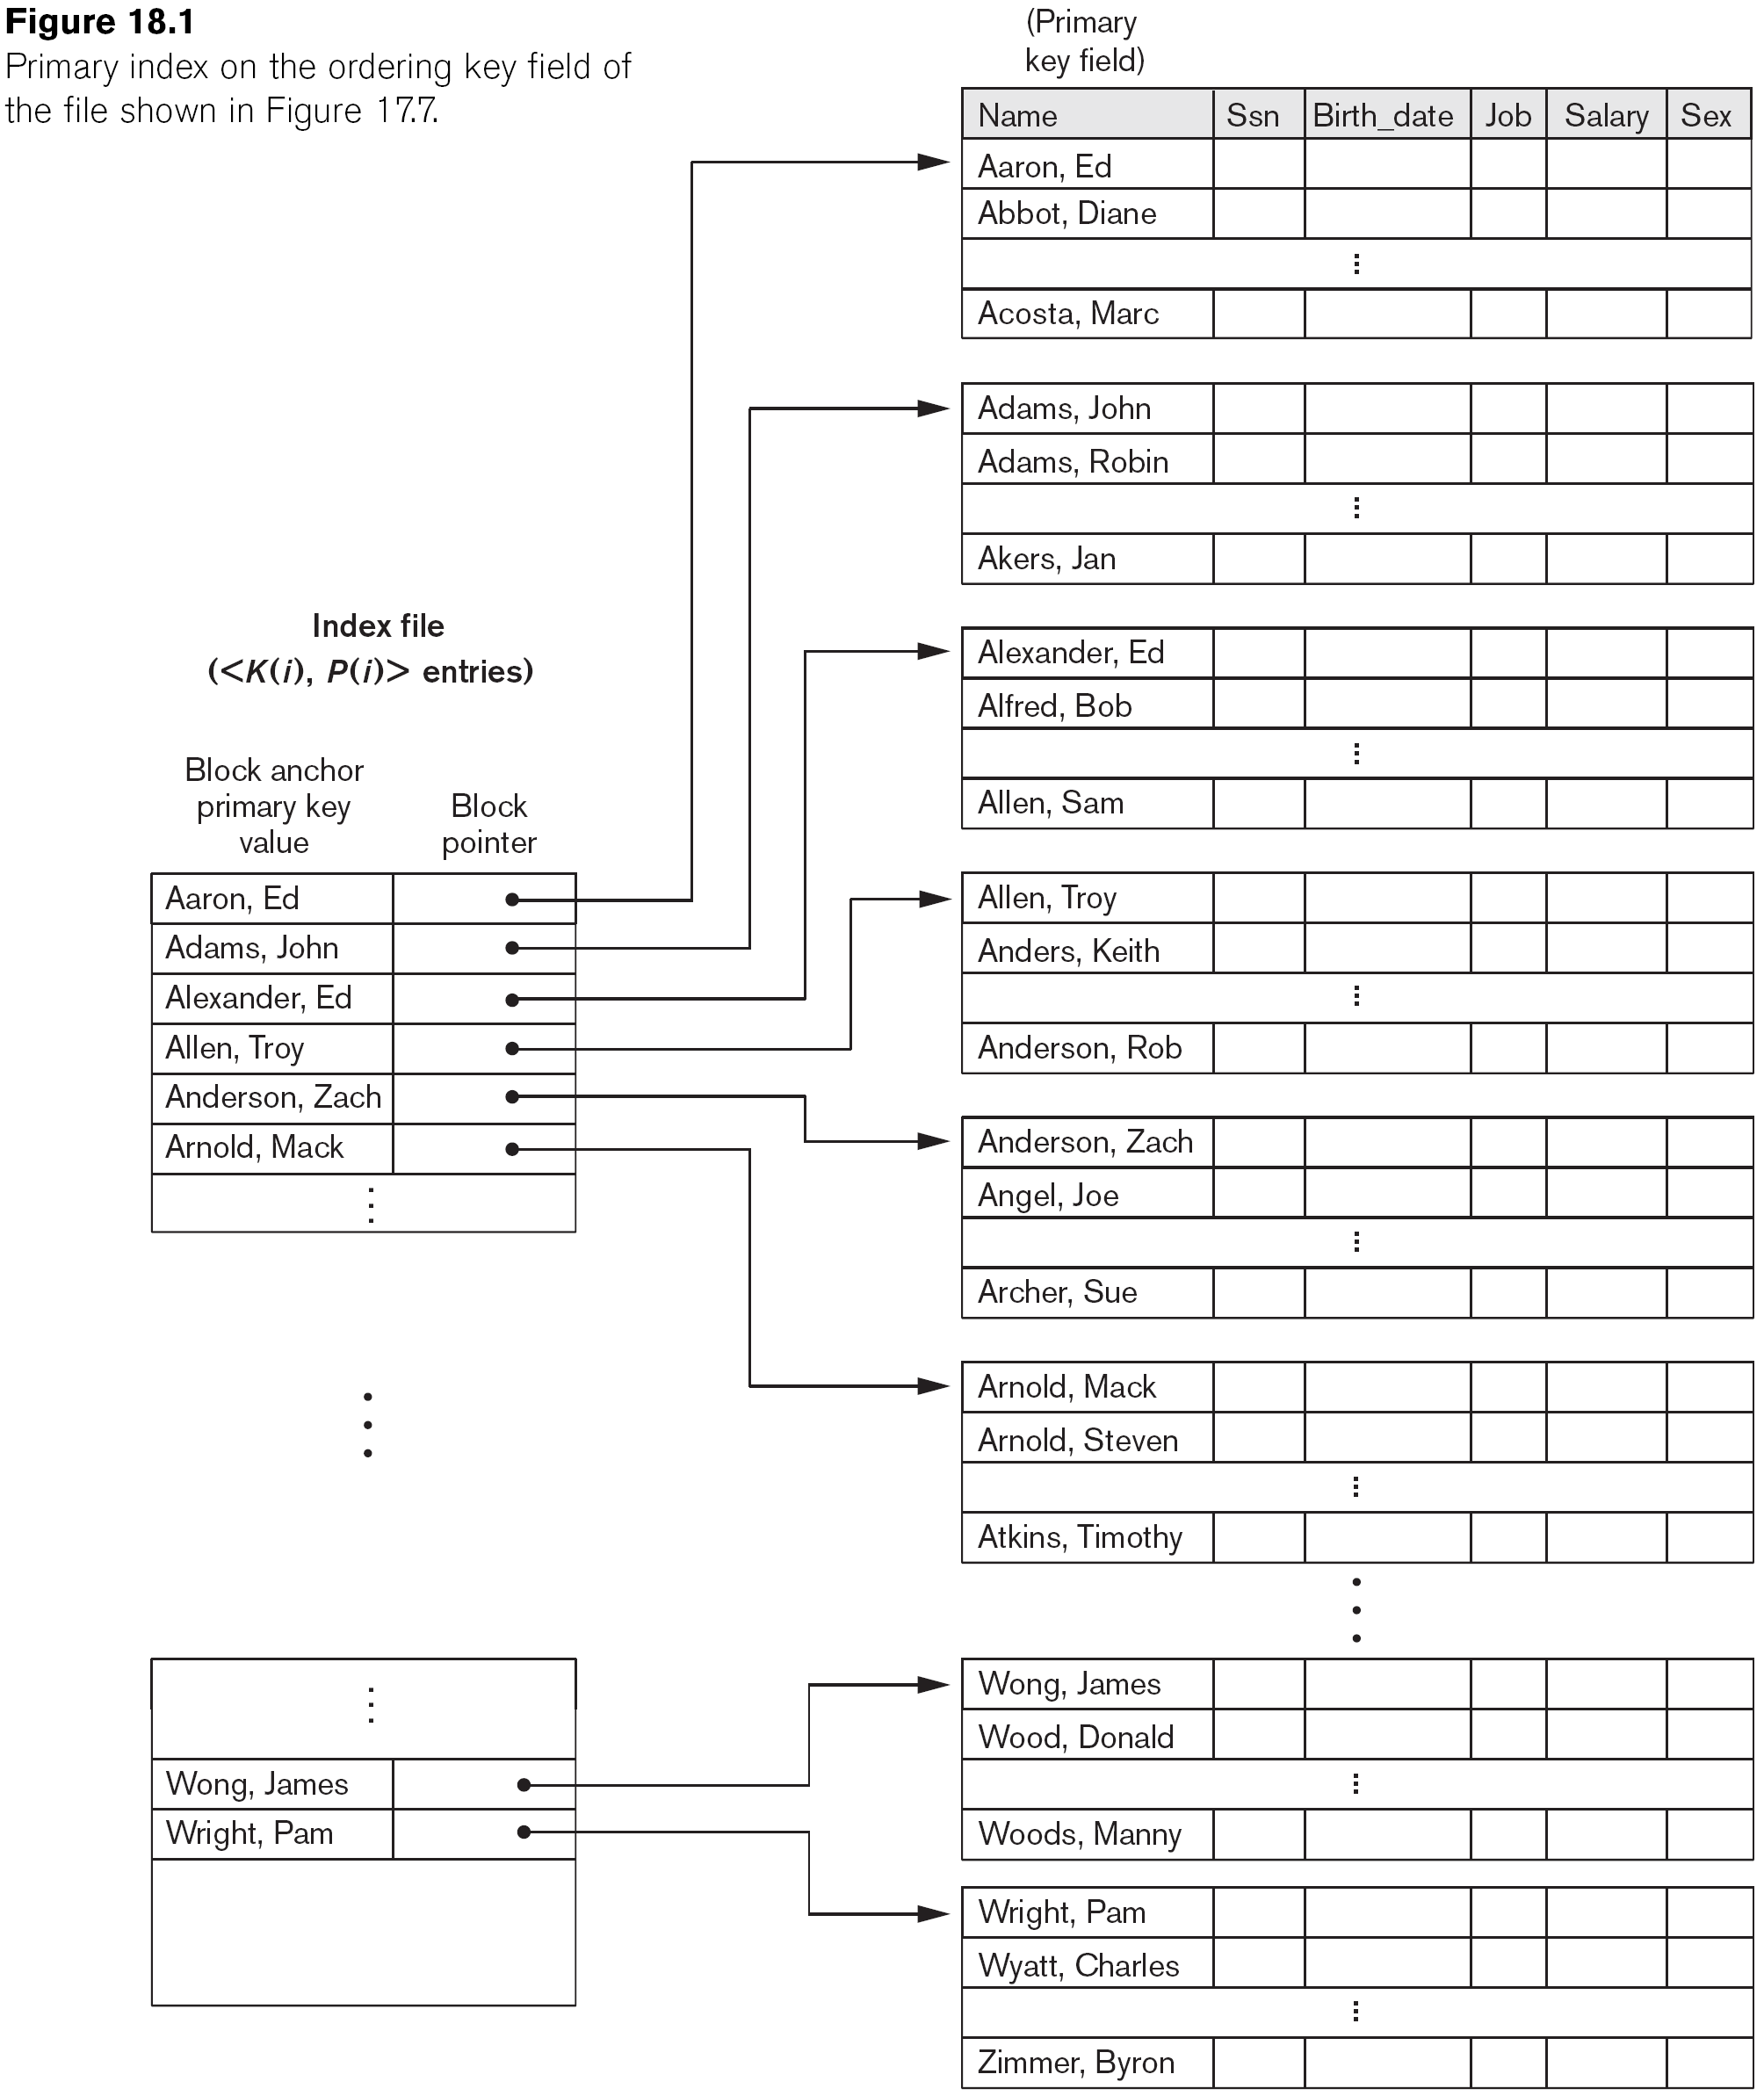
\includegraphics[width=6cm]{img/primary.png}
\end{tabular}

\subsubsection{Clustering index}
\begin{tabular}{m{7cm}m{8cm}}
\begin{itemize}
    \item The data file must be ordered on a non-key field (cluster field)
    \item One index entry for each distinct value with that field value
    (block pointer points to the first occurence of this value)
        $\to$ \textbf{sparse index} 
\end{itemize}
&
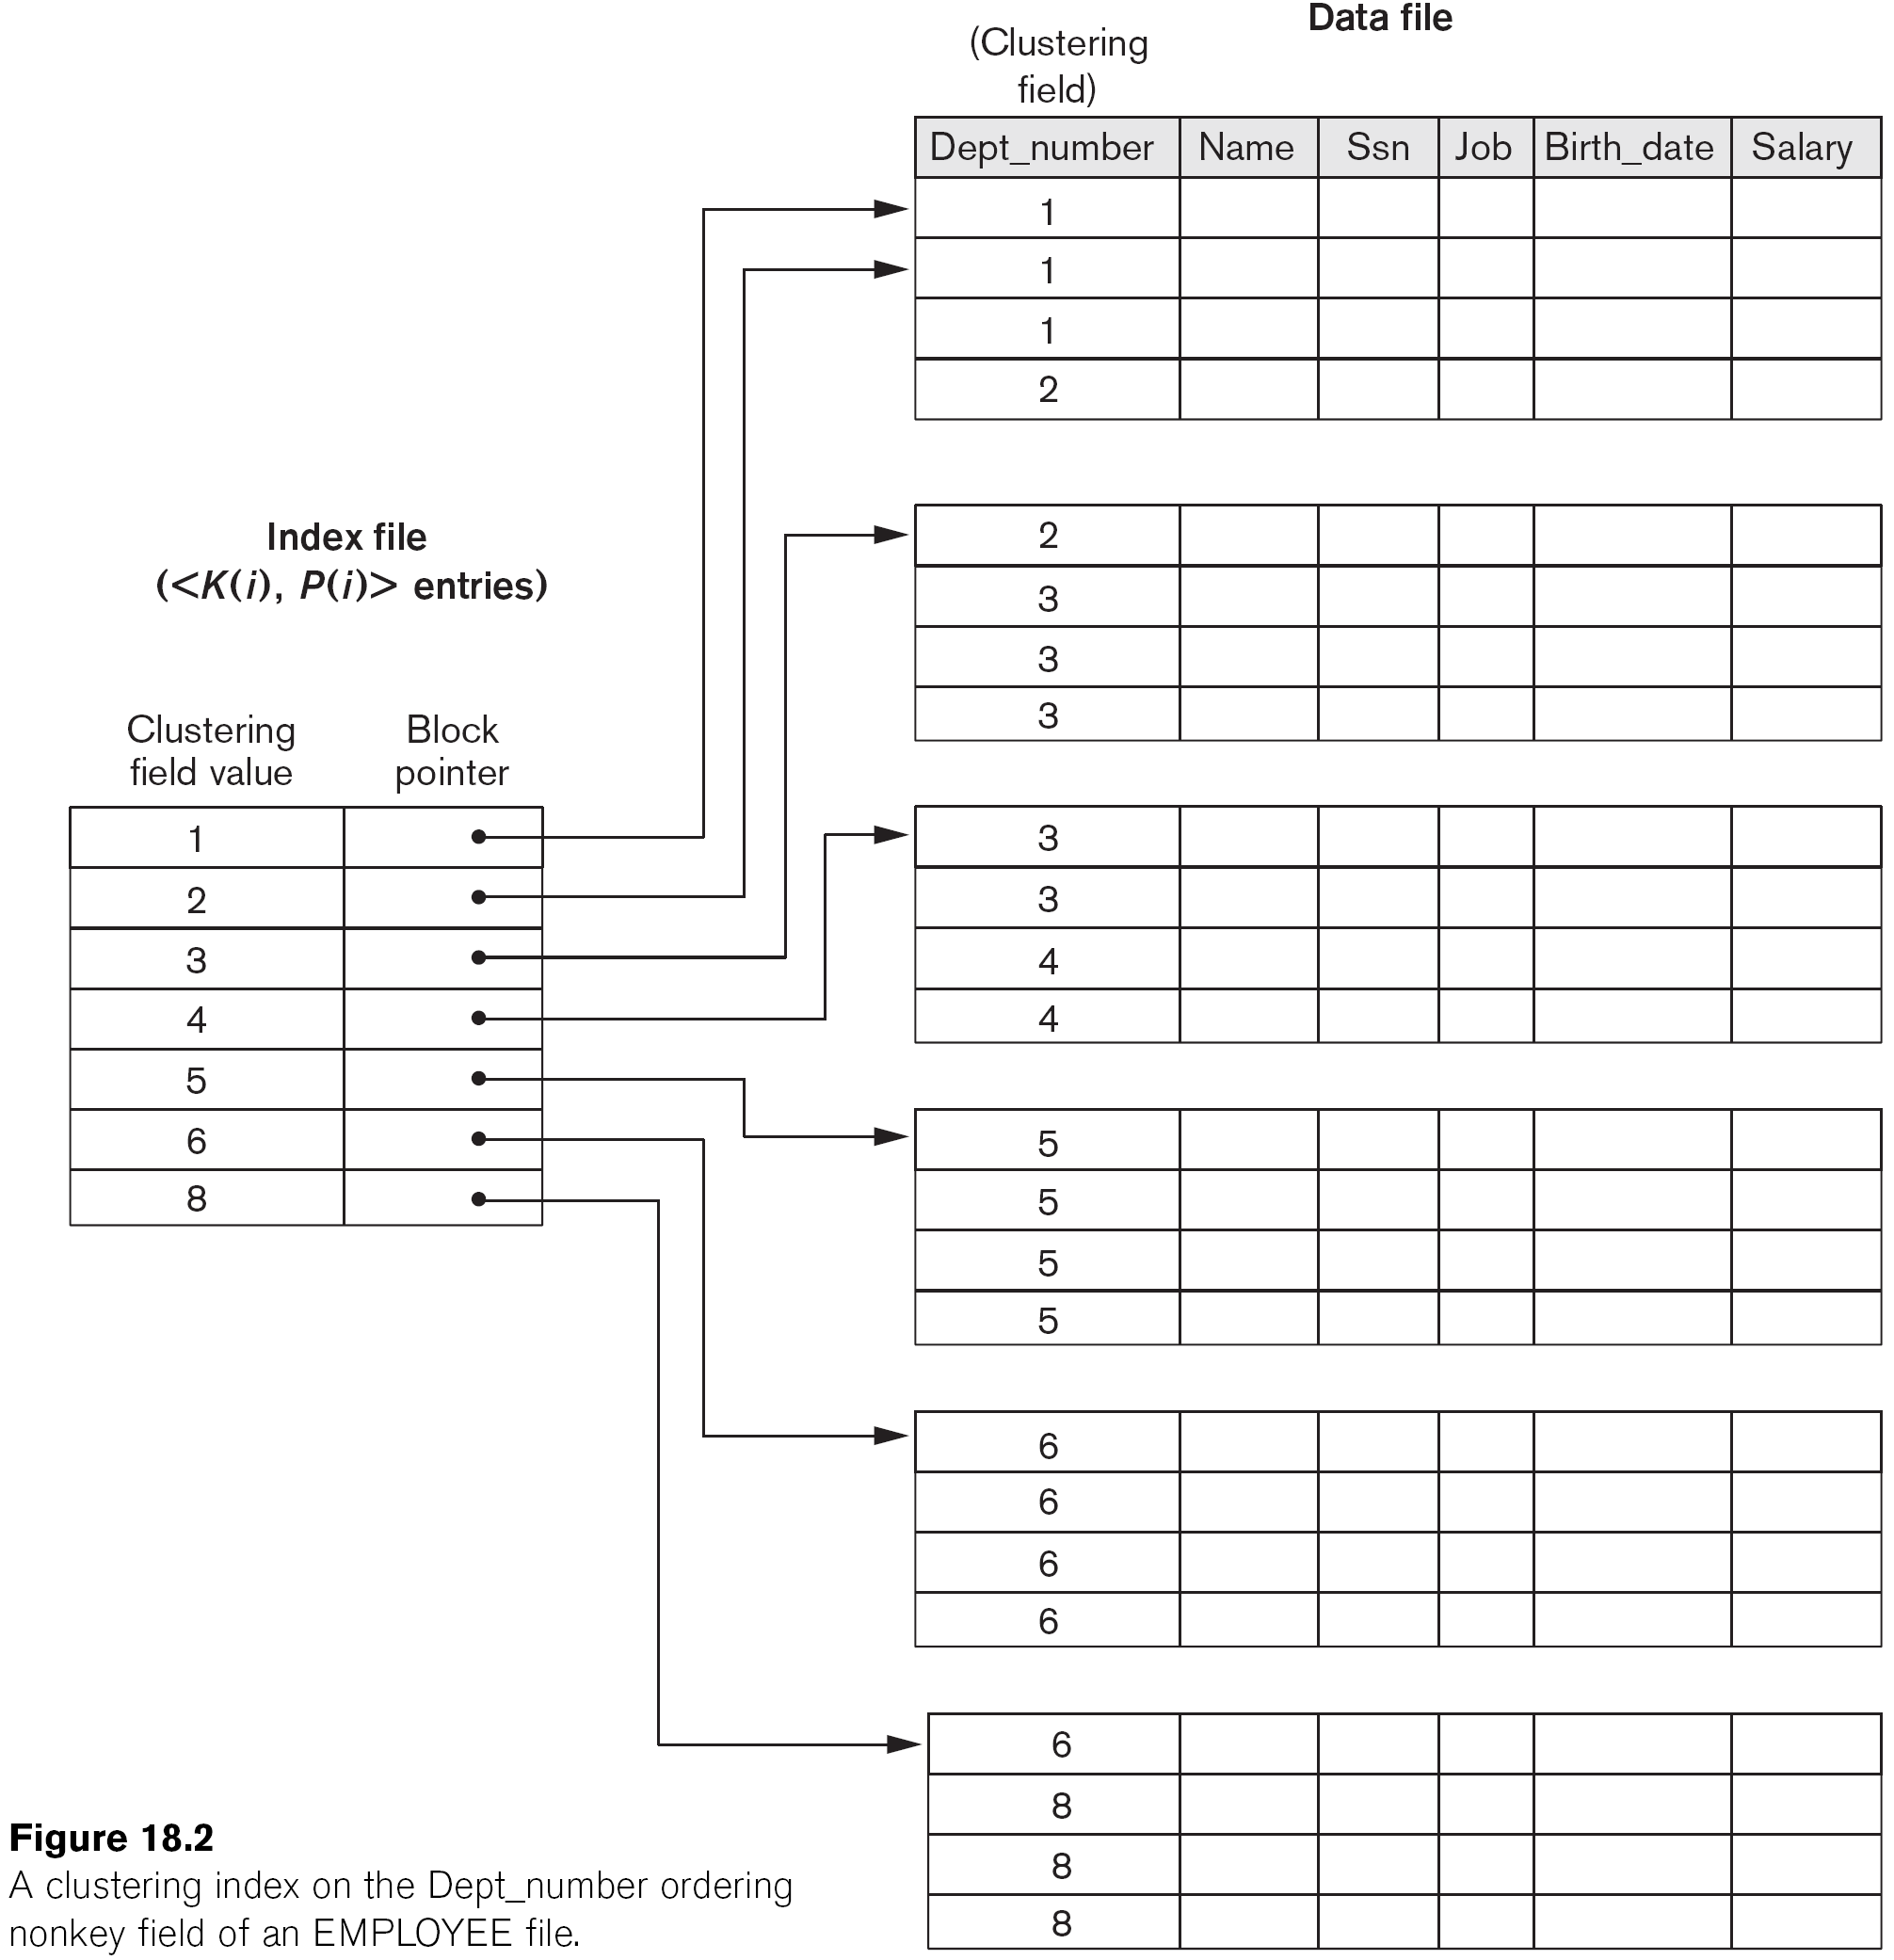
\includegraphics[width=6cm]{img/clustering.png}
\end{tabular}

\subsubsection{Secondary index}
\begin{tabular}{m{7cm}m{7cm}m{7cm}}
\begin{itemize}
    \item Accessing a file for which some
        primary access already exists.(can be several for the same file)
        \begin{enumerate}
            \item With a candidate key
            \item or a non-key with duplicate values
        \end{enumerate}
    \item Composed of two field : data type and (block pointer or recorde pointer)
    \item One entry for each record $\to$ \textbf{dense index}
\end{itemize}
&
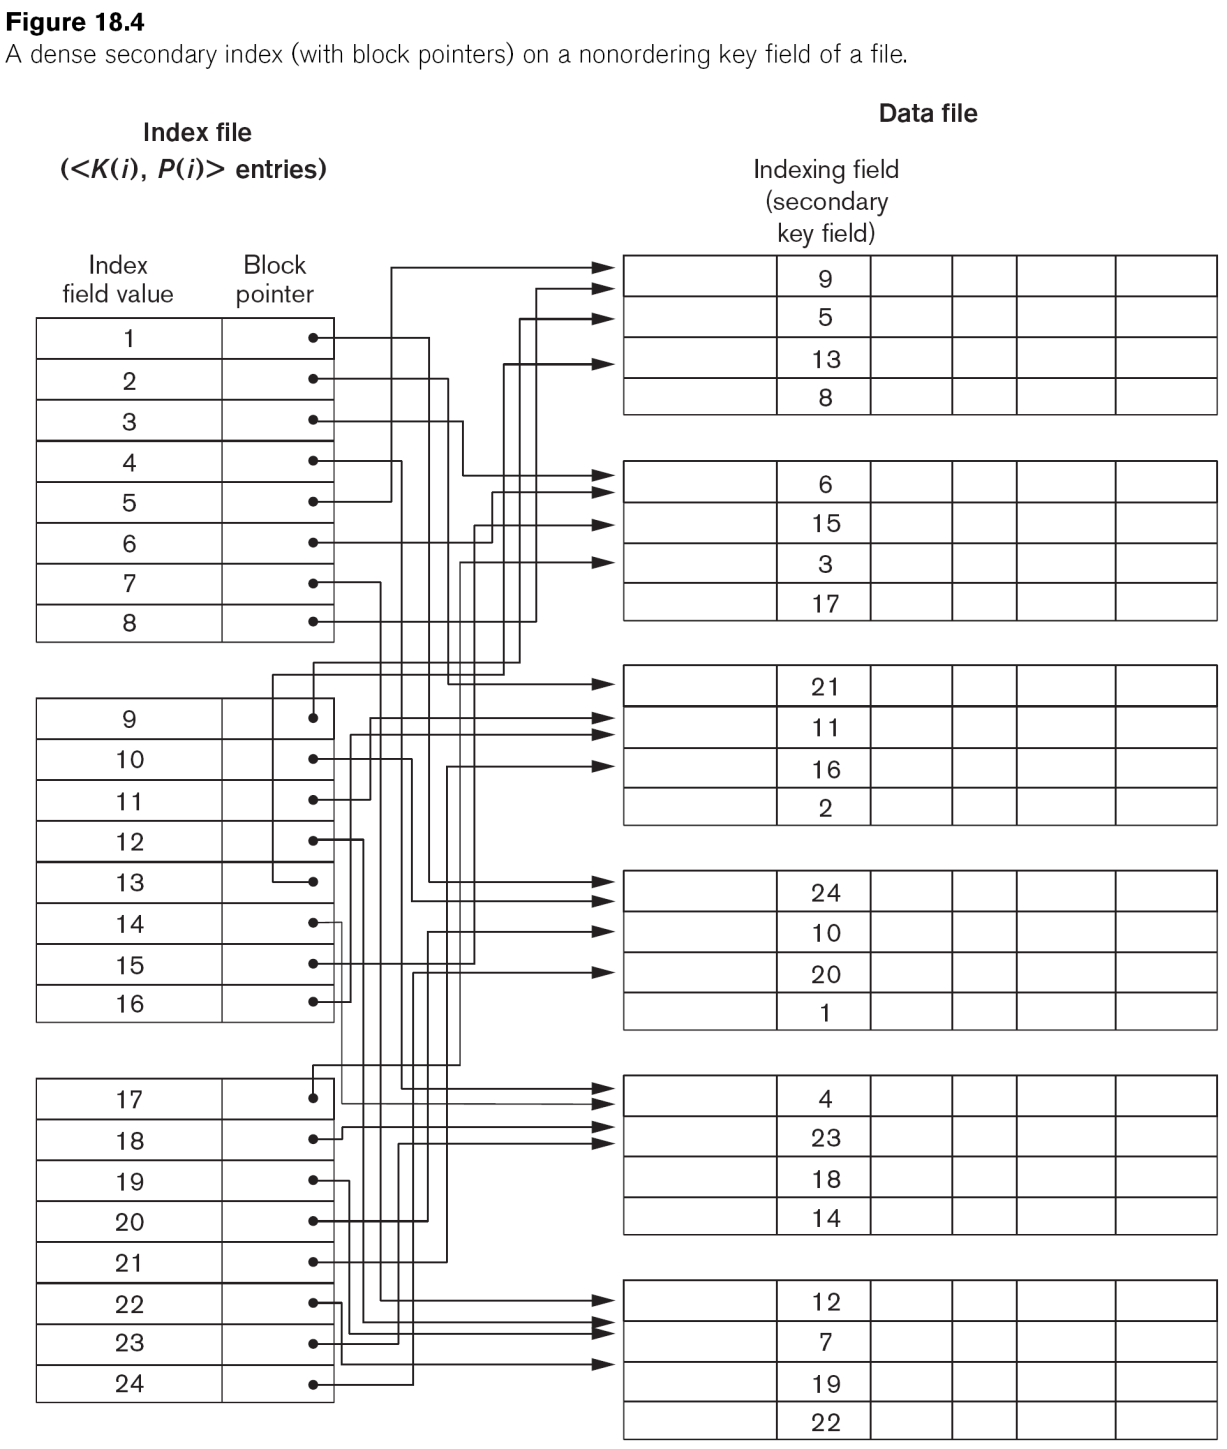
\includegraphics[width=6cm]{img/secondary1.png}
&
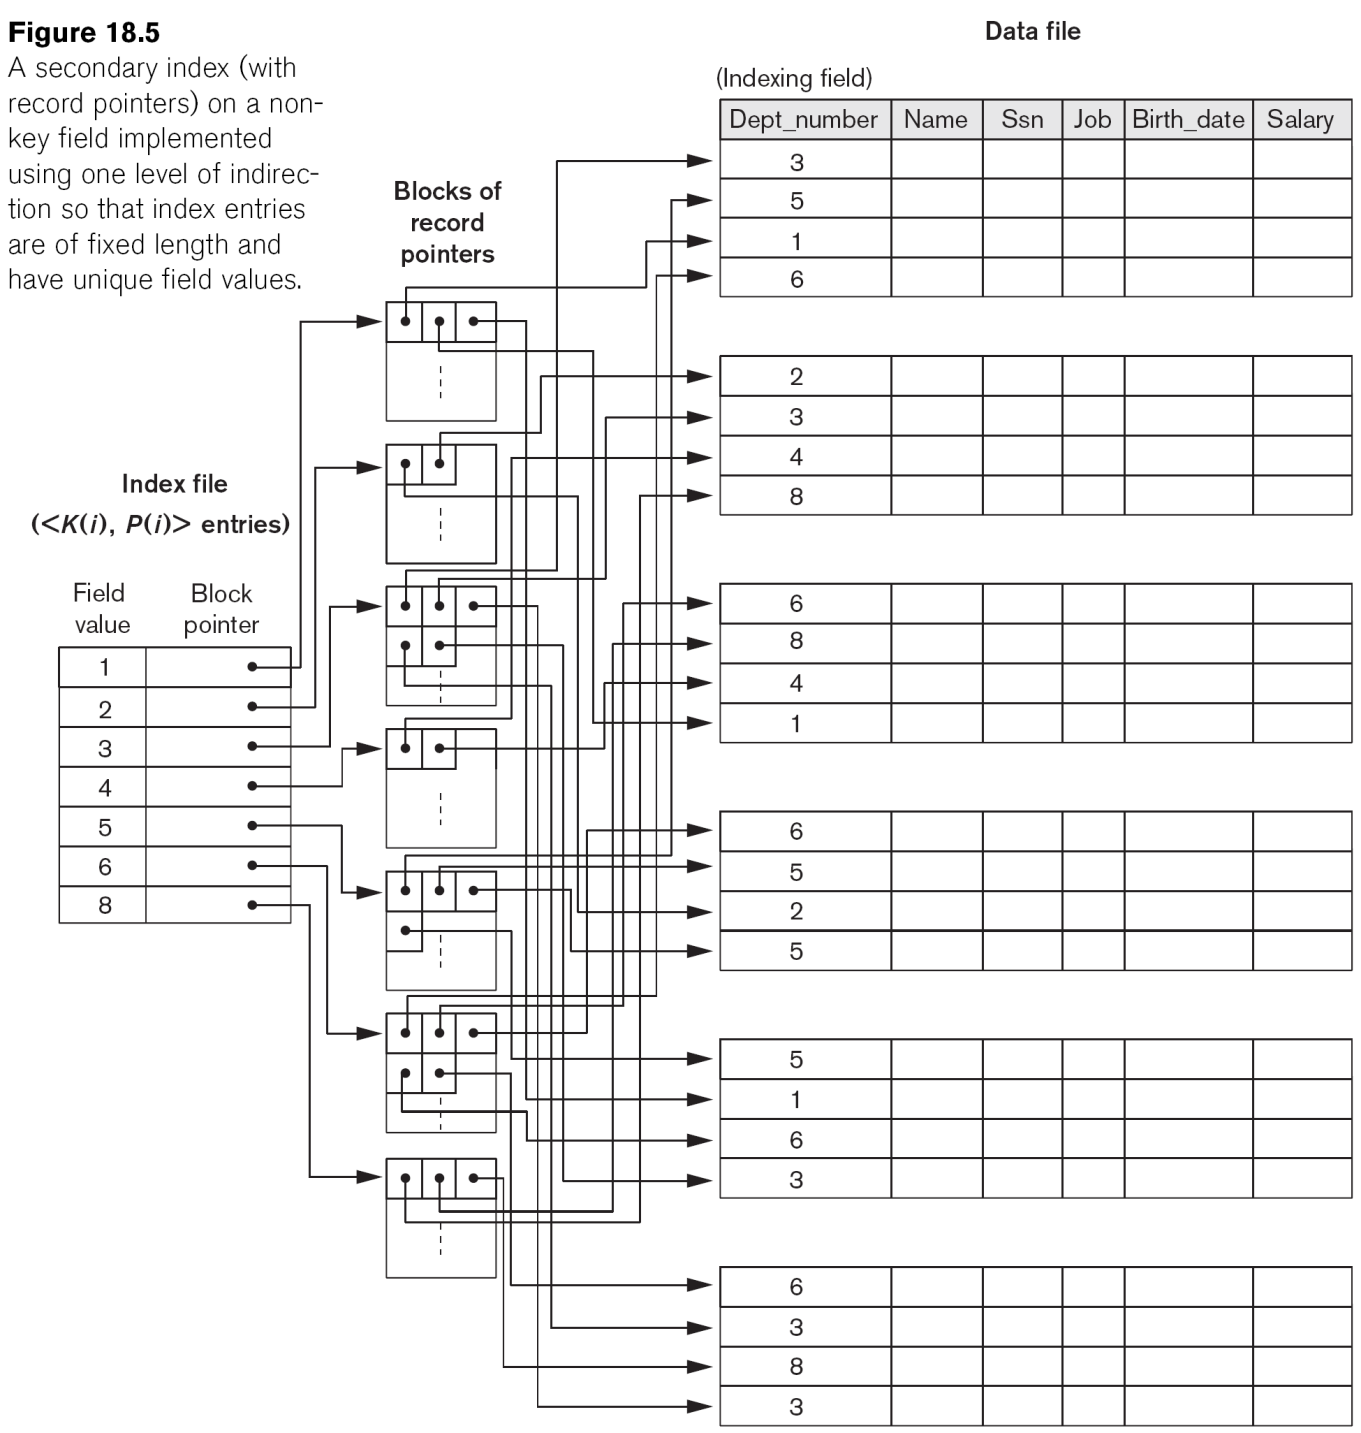
\includegraphics[width=6cm]{img/secondary2.png}
\end{tabular}

\subsubsection{Multi-level index}
\begin{tabular}{m{7cm}m{8cm}}
\begin{itemize}
    \item Multi-level index is done with a B-Tree data structure
        by repeat a primary/clustering index on multiple level 
    \item[]
    \item[Remarque:] Multi-level is is useless if add levels don't separate they element in
        different block
\end{itemize}
&
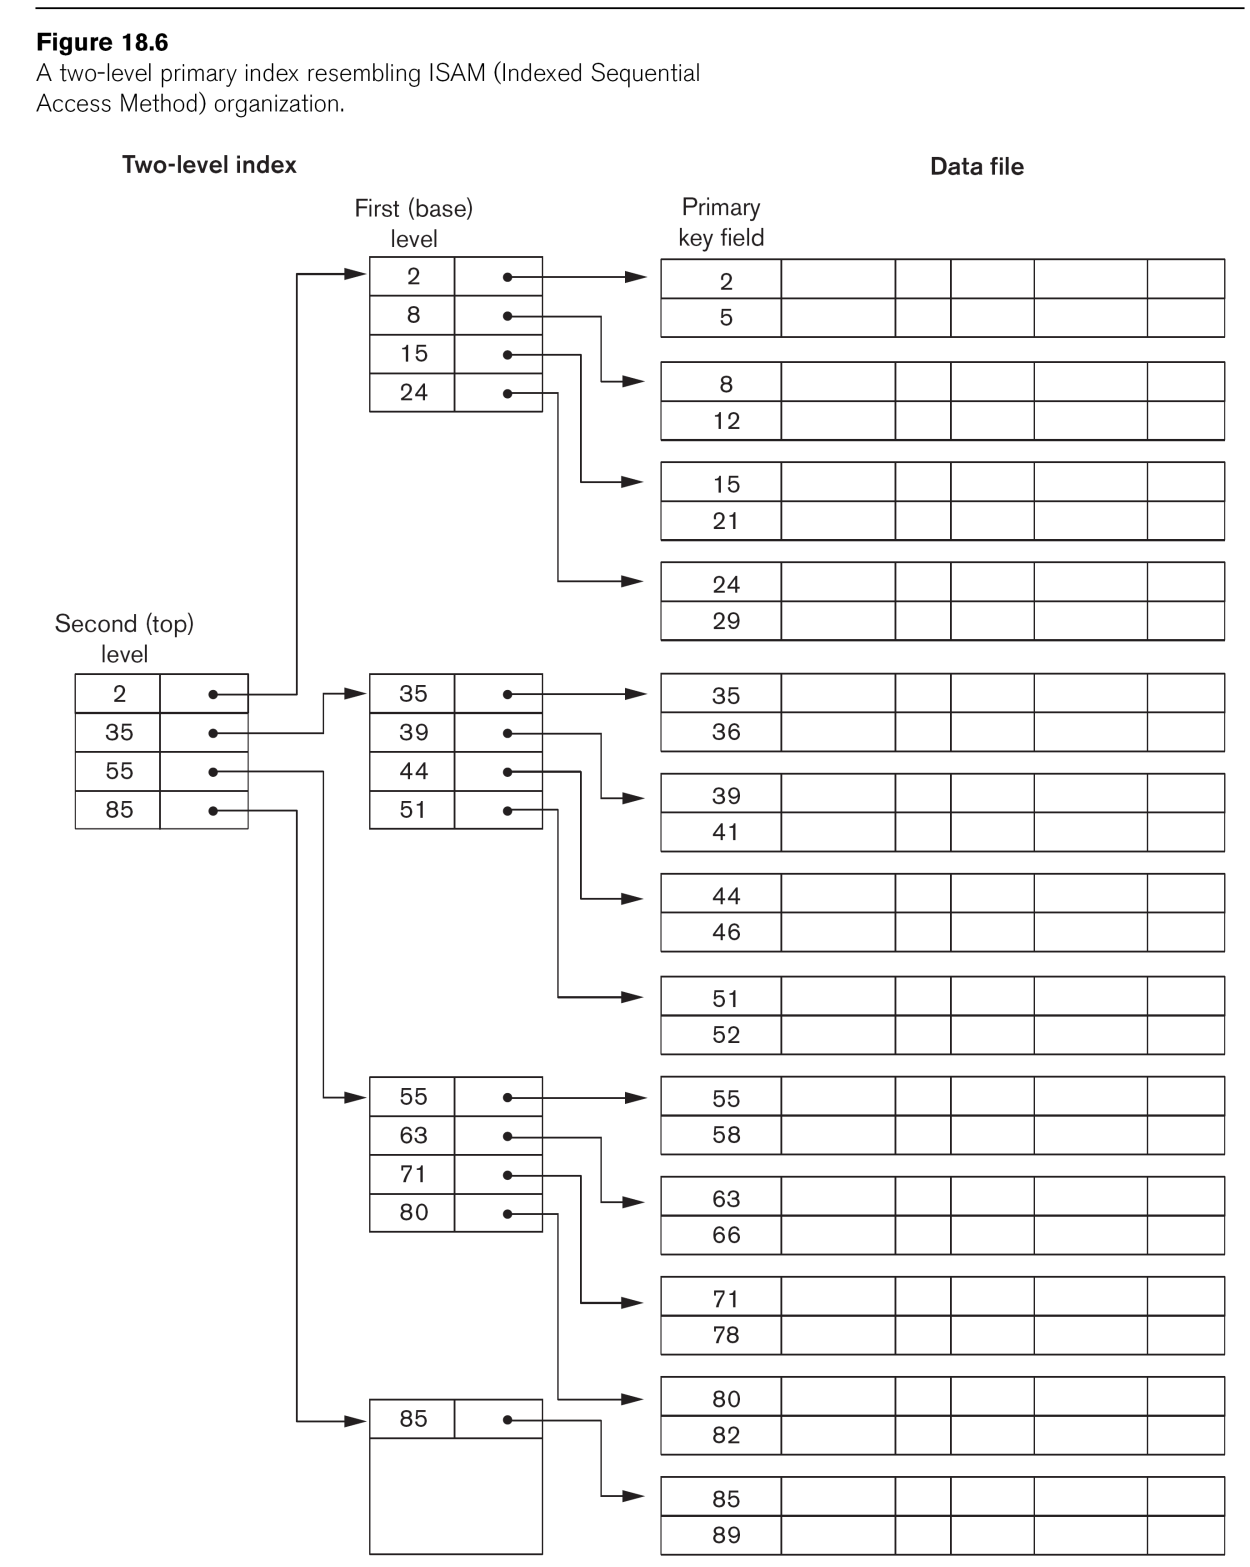
\includegraphics[width=6cm]{img/multi.png}
\end{tabular}


\paragraph{B-Tree and B+-Tree}

%TODO quick explanation on how B tree work

\begin{figure}[!h]
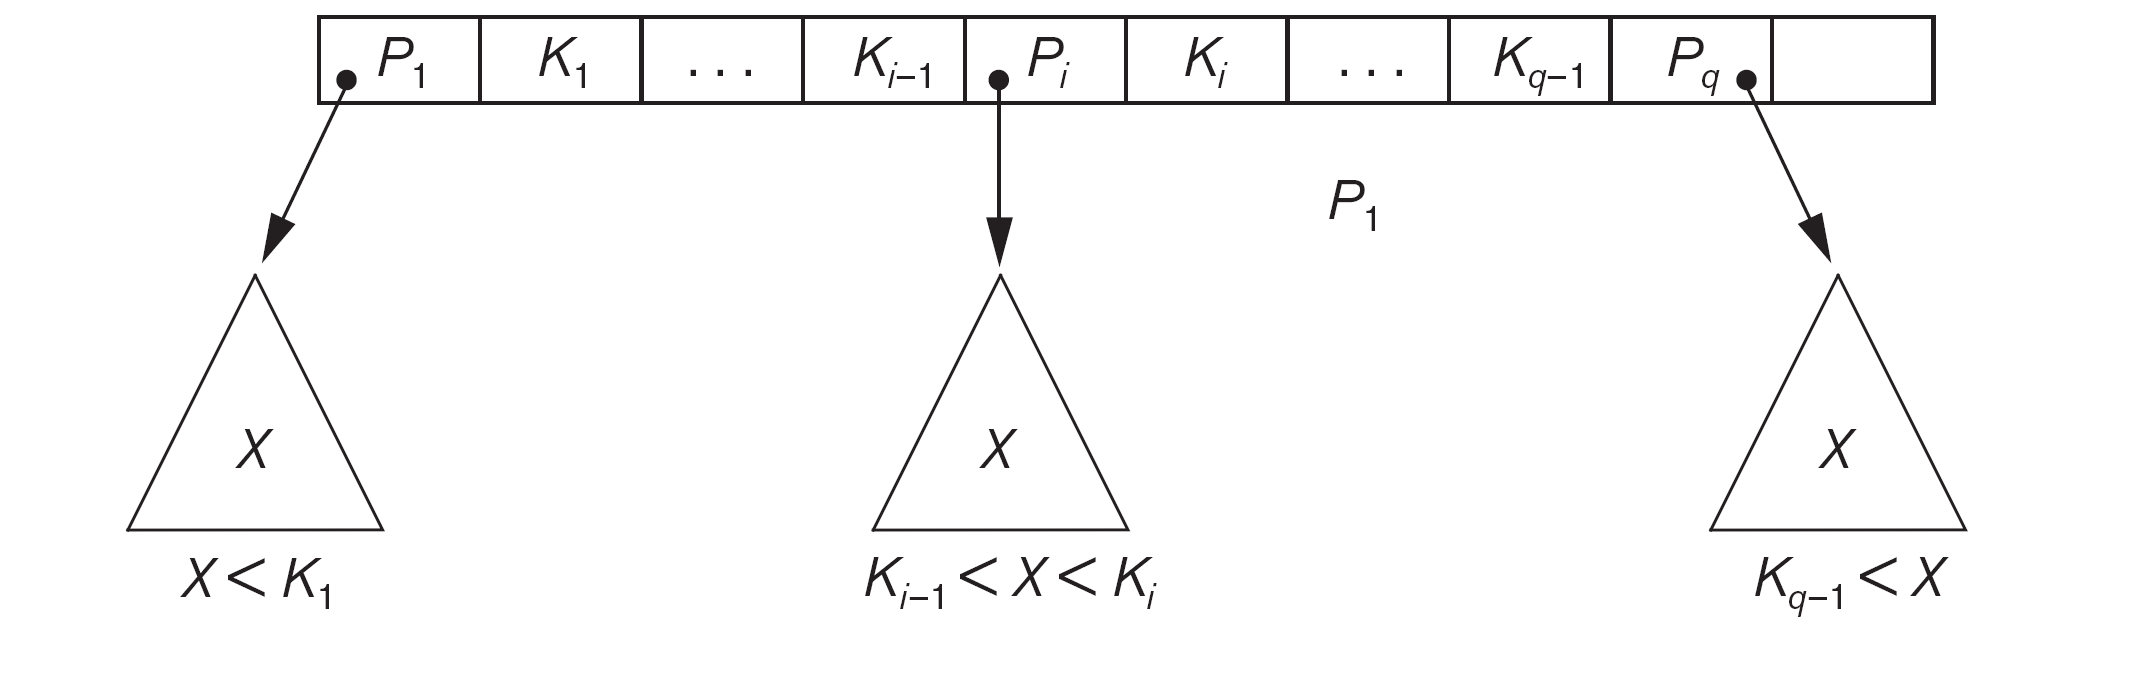
\includegraphics[width=6cm]{img/btree.png}
\caption{B-tree}
\end{figure}

B-Tree solve the problem to insert and delete new entries in
a multi level which must be ordered. (In this data-structure
these operation are quite efficient)

\begin{itemize}
    \item Insert element in a node an split it in two node if the 
        node is full (Splitting may propagate to other levels)
    \item Deleted element from a node and if he become less than
        half full merged it with neighboring nodes.
\end{itemize}


\paragraph{ } B-Tree are pointers on \textbf{all level} of the three
where B+-Tree are pointer only at the \textbf{leaf level}

\subsubsection{Using indexes}
%TODO ?

\section{Query processing}
\begin{description}
	\item[Query processing] The process of translating from a high-level
	query language to actual data access.
	\item[Query optimization] The process of choosing a suitable execution
	strategy for processing a query.
\end{description}
Two internal representations of a query : Tree or Graph.

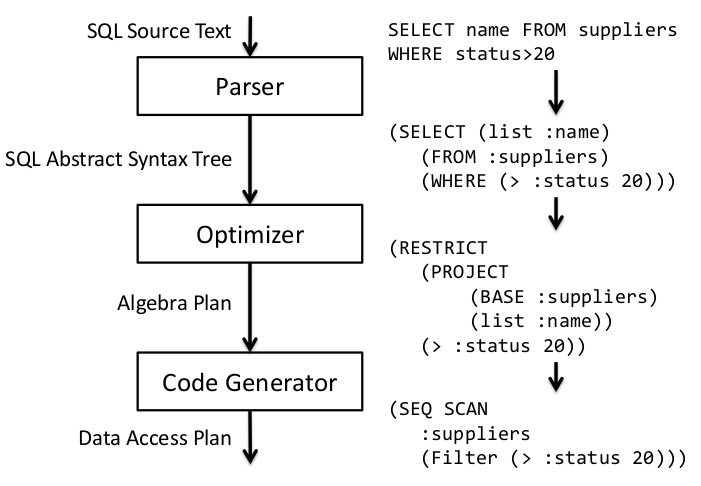
\includegraphics[width=9cm]{img/query.png}

\subsection{SQL $\to$ Relationnal algebra}

Query block (Single SELECT-FROM-WHERE [GROUP BY] [HAVING]) is the basic unit
that can be translated into \textbf{algebraic operator}.\\
Nested query within query are indentified as separate query blocks.

\subsection{Relationnal algebra $\to$ Data access}
For every abstract algebra operator (RESTRICT, PROJECT, JOIN,\ldots),
various algorithms exist (Sort-driven, hash-driven, loop-driven).

\subsubsection{External Sorting}
\begin{itemize}
	\item External sorting refers to sorting algorithms that are suitable for 
	large file of records on disk that do no fit in main memory.
	\item It uses sort-merges strategy, it consist of sorting small subfiles
	(runs) then merges them.
	%TODO cost?
\end{itemize}
\subsubsection{Restrict}
There are diffent algorithm that can be use to implement the restrict
\begin{itemize}
	\item Linear search: Check on every record, if it satisfy a condition
	\item Binary search : If restriction condition involves
	 a equality comparison on a key attribute and the file is ordered.
	\item Primary index (or hash key) : if restriction condition involves
	equality comparison on a key attribute witth a primary index.
	\item Primary index to retrieve multiple record: If there is a 
	comparaison condition other that = on a key field with primary index.
	\item Cluster index to retrieve multiple record : Restriction 
	involves an equality comparison on a non-key attribute with clustering
	index.
\end{itemize}
If the condition involves only one attribute , the brute force linear 
search is used if there is no access path.\\
If the condition involves many attributes, it's the role of the query 
optimization to choose the best access path. 

\subsubsection{Join}
Different techniques to implement the join
\begin{itemize}
	\item Nested-loop join : Test the join codition t[A] = s[B] for every pair 
	of record (where A and B are domain-compatible attribute and t and s
	are record for R and S).
	\item Single-loop join: If a index exists for one of the two join
	attributes, use access structure to retrieve all matching records
	that satisfy join condition.
	\item Sort-merge join : %TODO
	\item hash-join : %TODO

\end{itemize}

\subsubsection{Project}
%TODO
\subsubsection{Set}
%TODO
\subsection{Pipelining Operations}
%TODO
\subsection{Query Optimization}
%TODO

\section{NoSQL}

No SQL has been created to answer the problem of the scalabilility/
velocity/volume of data.  Goal is not replace RDBMS but rather act
as a complement.\\
Oriented on aggregate which is a collection of related objects that 
treated as a unit.\\
There are four basic type of database:
\begin{description}
	\item[Key/value]: Similar to a hashmap. Data are represented by 
	key/value couple. All intelligence is left to the querier. Basic 
	operation are : PUT,GET,DELETE.
	\item[Column-family Stores]: The number of column is variable. It allows
	to avoid NULL value. To achieve this variation in the number of column,
	many columns are associated with a row key.
	\item[Document] Based on the key/value paradigme. Value is a document
	(JSON or XML). It's easy with only the key , to get information 
	organized in a hierarchical way.
	\item[Graph] Entities are stored as node and relation are depicted via
	the edges.
\end{description}
\url{http://blog.neoxia.com/nosql-5-minutes-pour-comprendre/}

\subsection{Data Distribution}
%TODO

\section{Other Material}
\subsection{S3}
Pour l'union, elle est bien commutative (on s'en fout du résultat et du truc bizarre sur SQL, la question c'est "est-ce que l'union est commutative").

\subsection{S4}
Voir mémoire.

\subsection{S5}
On peut utiliser un \texttt{EXTEND}:
\begin{lstlisting}
EXTEND NOM_DE_LA_TABLE : {NOM_NOUVELLE_COLONNE}
EXTEND SUPPLIERS : {TOTAL := COUNT(SUPPLIERS), TOTAL2 := COUNT(PARTS)}
\end{lstlisting}

\subsection{S9}
EER: Enhanced Entity-Relationship Model, a high-level conceptual data model extended from the Entity-Relationship Model. Source: Kikipedia (\url{https://en.wikipedia.org/wiki/Enhanced_Entity-Relationship_Model}). ER est en top-down.

%\begin{center}
%	\includegraphics[width=.75\textwidth]{pub2.png} % merci Ben :)
%\end{center}

\subsection{A bottom-up design method}
 The bottom-up approach begins with the specific details and moves up to the general.  To begin a bottom-up design, the system analyst will inspect all the interfaces that the system has, checking reports, screens, and forms.  The analyst will work backwards through the system to determine what data should be  stored in the database.\\

To understand the differences between these approaches, let's consider some jobs that are bottom-up in nature.  In statistical analysis, analysts are taught to take a sample from a small population and then infer the results to the overall population.  Physicians are also trained in the bottom-up approach.  Doctors examine specific symptoms and then infer the general disease that causes the symptoms.\\

\subsection{Database designs}
\subsubsection{Le meilleur}
Ça dépend toujours du design...

\subsubsection{With respect to real-world requirements}
\todo{Julien}

\subsubsection{Underlying objectives}
Les NF aide à faire ça
\begin{itemize}
  \item Avoid Redundancy: Si on a du 5NF, on évite la redondance car
  \item Update Anomalies: Pas en 6NF
  \item Achieve Simplicity: En 6NF
  \item Orthogonality: (plus c'est séparé, plus c'est orthogonale), ex: 6NF (peut-être même trop)
\end{itemize}

\subsubsection{Typical exam question}
\todo{TODO: Julien}
L'oracle sert à prédire le reste.\\
Décomposer R en R$_1$ ... R$_n$ en BCNF: voir définition de BCNF, c'est le match de la Suisse en ce moment... (\textit{Il faut que la clé implique}). \textbf{Il y a un algo dans les slides}.\\
Tutorial D: voir match Suisse -- Equateur.

\section{Exam}
\subsection{Expliquer pourquoi l'implémentation des views dans PostGreSQL brise la règle de Logical Dependencies}


\subsection{Donner les avantages et inconvénients des databases JSON suivant certains requirements}
\begin{itemize}
	\item Communiquer directement avec la DB).
    \item JSON comme une base de données (like NoSQL). Mais ce n'est pas relationnel -> c'est la merde de mettre ca dans un type de base de données relationnel (pas 1NF)
    \item compare c'est la merde
    \item si tu chopes un JSON pour ta DB, tu peux le save
    \item si TYPE en REL, on peut ajouter des opérateurs
\end{itemize}

\subsection{Atomicity of ACID}
La transaction est vue comme une seule transaction, même si elle est constituée de plein de petites transactions. Donc, l'atomicité consiste à voir une trnsaction comme si c'était une seule opération. De ce fait, soit la transaction réussi et est effectuée, soit la transaction plante et donc, rien n'est fait (comme si on avait pas fait de tansaction).

Pour assurer l'atomicité (quand une transaction plante) :
\begin{itemize}
  \item Undo log : reverse action déjà faites
  \item Redo log : je retente les actions déjà faites
  \item mélange de undo/redo : je fais une soupe
  \item rollback/checkpoint : plus nouvelles transactions.  Quand fini, checkpoint (sauve DB) et je reviens la si c'est la merde
  \item Backup DB : j'utilise mon backup
\end{itemize}

\subsection{Consistant of ACID}
Les contraintes doivent toujours être vérifiées.\\
Commit se fait que si toutes les contraintes sont vérifiées.\\
Rollback on revient au dernier état consistant.\\
\subsection{Isolation of ACID}
Toutes les transactions sont serializable ().\\
Implémenté avec des LOCK.  Read Only et Write Only.  Toujours dans le même ordre sont pris les lock.\\


\subsection{Les DB sont basées sur la théorie des ensembles.  Montrez le dans l'algèbre relationnelle}
Les types sont des ensembles de valeurs.\\
\texttt{NOT MATCHING} (disjonction), \texttt{MATCHING} (intersection), \texttt{WHERE} (appartenance)

\subsection{Pourquoi certaines versions de SQL ne permette pas d'updater les views ?}
Quand on update la view, on update pas les tables qu'elle utilise. Il faut créer une rule qui update les tables. Mais pas dispo dans toutes les versions.


\subsection{Index dans Postgresql}
Source: \url{https://dev.mysql.com/doc/refman/5.0/fr/mysql-indexes.html}.

Tous les index de MySQL (\texttt{PRIMARY}, \texttt{UNIQUE} et \texttt{INDEX}) sont stockés sous la forme de \texttt{B-tree}. Les chaînes sont automatiquement préfixée et leurs espaces terminaux sont supprimés.

En PostgreSQL, B-tree, R-tree, Hash ou GiST.

\subsection{Expliquer l'indépendance des données (logique et physique)}
Dépendance physique : Peut importante le support, ca doit toujours être la même représentation.\\
Dépendance logique : Dépendant dans l'idée mais pas la même entre la DB et le programme\\

\subsection{En quoi l'architecture ANSI-SPARC en est liée avec le data model}
Il s’agit de l’architecture fondamentale sur laquelle reposent les SGBD modernes, elle fut proposée en 1965 par Charles Bachman qui reçut le prix Turing pour ses travaux. L’architecture Ansi-Sparc est divisée en trois niveaux, celui du schéma interne (SI), celui du schéma conceptuel (SC) et celui des schémas externes (SE).\\
La première innovation de l’architecture Ansi-Sparc est la distinction claire entre la représentation interne des données au niveau physique (structure de données) et la représentation logique de celles-ci. Une base de données est définie et manipulée via le niveau conceptuel (SC) sans avoir à se soucier des détails de l’implémentation physique (SI). Par exemple, il est possible de définir un index sur un ensemble de données, mais comment celui-ci est réalisé au niveau physique n’a pas besoin d’être spécifié. Sur le même principe, lors d’une requête, l’usager n’a pas besoin d’indiquer comment utiliser l’index pour maximiser l’efficacité de la recherche.
La deuxième grande innovation de ce modèle est la possibilité de créer des schémas externes qui sont en fait des portions de la base de données (sous-bases virtuelles) destinées à différents usagers. Un usager particulier ne peut manipuler que les données appartenant à son propre schéma externe. De nos jours, le terme schéma externe est remplacé par celui de « vue ».\\
\subsection{Définir une relation et donner le lien avec le first order logique}
une relation c'est un ensemble de tuple qui vérifie une propriété.\\
Le first order les prédicats qui peuvent être instanciées en fonction des variables (soit vrai soit fausse) et au final la propriété peut être un prédicat.  Les tuples pouvant être acceptés sont ceux qui vérifient un prédicat.\\
Closed world assumption : l'entièreté des tuples peuvent être mis dans la relation.  On suppose que la relation a tous les tuples.
\subsection{BCNF}
Table donnée.  Créée une nouvelle relation.  Pourquoi pas BCNF ?  FD uniquement trivial ou X super Key.  Or, ici cours est toujours=C1.  FD Point vers cours et point n'est pas superkey, donc merdoum.
\subsection{Requete et le query plan donné.  Que fait l'optimizer ?}
Associativité : restriction sur chaque avant de join.\\
Mettre un clustering index et un index primaire sur les quantités.

\subsection{Question Vincent}
\subsubsection{Requête}
1 question avec une requete à faire, et dire comment j'aurais pu faire pour la mettre comme contrainte dans ma DB en tuto D. Et aussi en SQL. La question c'etait genre, dans l'exemple suppliers, shipments, parts s'assurer qu'un fournisseur localiser à Paris ne puisse pas founir plus de 3 parts différentes. je fais le summarize et je dis where countPID > 3 et je dis que ca dois etre = TABLE\_DEE. Pour sql j'ai récris la requete et j'ai dis qu'il faudrait mettre dans un trigers qu'il verifie la contrainte a chaque fois qu'un shipment est insérer $\Rightarrow$ faut une rules plutôt!

\subsubsection{closed world assumption}
"closed world assumption" in database field et expliquer en quoi c'etait relié à la théorie des prédicats dans la logique du premier ordre. $\Rightarrow$ Closed pour 'fermé'. Venant de Kikipedia:

La notion d'hypothèse de monde clos est utilisée en particulier en Prolog, elle s'oppose à l'hypothèse de monde ouvert (voir aussi l'article Logique argumentative) et concerne la question du vrai et du faux.

Elle signifie qu'un fait est considéré comme faux si, en un temps fini, on échoue à montrer qu'il est vrai, ce qui revient à dire que tout ce qui est vrai doit être connu (inclus dans la base de données des faits) ou démontrable en temps fini, il n’y a pas de monde extérieur qui pourrait contenir des éléments de preuve inconnus du programme. Pour les faits vrais, l'hypothèse de monde clos ne dit rien de particulier.

Avec l'hypothèse de monde clos, l'univers des faits se partage entre les faits 'vrai' prouvables en temps fini et tout le reste, assimilé au faux (pour ce qui est accessible en temps fini). Outre la question de la terminaison, cela impose une utilisation du 'faux' avec précaution. Autant le 'vrai' est fort (il ne dépend que de la base de faits et de règles initiale acceptée et du mode d'inférence adopté), autant le 'faux' dépend de l'exhaustivité de la base de faits et de la complétude de la base de règle (2 notions délicates à obtenir).\\

Relation avec la DB: This 1:1 correspondence reflects the Closed-World Assumption:
\begin{itemize}
	\item A tuple representing a true instantiation is in the relation.
	\item A tuple representing a false one is out.
\end{itemize}
(and vice-versa, with respect to the database vs. the world)
The Closed-World Assumption underpins the operators we are
about to meet.
i.e. Algebra operators do not create new facts out of nowhere

\subsubsection{ACID}
il me demandait d'expliquer ce qu'etais l'atomicité d'une transaction et comment on pouvait implementer ca

j'ai dû définir relation et faire le lien avec la logique du premier ordre

\subsection{Question Ricetti}

ACID

une question de porc sur un algo rela que jai pas su faire mais le prof ma dit que cetaitt la plus dure de tte les question
KeRANK r { a1 , a2 , a3 ,... ak }

\subsection{INSERT/DELETE/UPDATE sont des shorthands pour une assignation de relvar}
Shorthands pour raccourcis je suppose...
\begin{itemize}
	\item INSERT, for adding tuples to a relvar
	\item UPDATE, for updating existing tuples in a relvar
	\item DELETE, for removing tuples from a relvar
\end{itemize}

\subsection{Comment optimiser les DB qui tiennent entièrement en RAM}
Que mettre dedans? Si on doit choisir, d'abord l'index. Si c'est tout, faut-il optimiser le temps d'accès ou la place? Et donc en gros, répondre à: comment arranger les info?\\
Vu que c'est du random access memory, on s'en fout où c'est en mémoire (toujours le même temps d'accès, peu importe où on doit aller).
\begin{itemize}
	\item Si on doit minimiser la place, vaut mieux éviter plein de références et avoir tout en un bloc (si on sait que la suite est juste après, pas besoin d'utiliser de la mémoire pour dire que le bloc suivant est à l'adresse X, ça occupe de la place...  $\Rightarrow$ donc plus dans l'idée d'utiliser surtout un primary index (voir multi-level pour profiter des B-Trees) et donc un \textit{sparse} index pour avoir une index que sur qqs search values.
    \item d'un autre côté si on veut optimiser le temps d'accès, c'est intéressant d'avoir plein de jumps pour éviter de tout lire et directement avoir ce que l'on veut surtout que le coût des jumps en terme de temps est (quasi) nul $\Rightarrow$ secondary Index et donc avec un index \textit{dense}: une entrée dans l'index pour chaque valeur recherchée.
\end{itemize}
Mais ça m'a l'air faible comme explication...\\
Pour moi l'idée est de profiter du temps d'accès ultra rapide peu importe où se situe l'info. Si on a plein de jumps, sur un disque dur, c'est lent.\\
Note: en RAM, s'il n'y a plus de courant... tout est parti!

\end{document}
